%------------------------------------------------
%	PACKAGES AND DOCUMENT CONFIGURATIONS
%------------------------------------------------
\documentclass[11pt]{article}
\usepackage{amsmath} % Required for some math elements
\usepackage{hyperref} 
\usepackage{xcolor}
\usepackage{lipsum} 
\usepackage{cite}
\usepackage{graphicx} % Required for the inclusion of images
\usepackage{algorithmic}
\usepackage{array}
\usepackage{bookmark}
\usepackage{listings}
\usepackage{amssymb}
\usepackage{enumitem}
\usepackage{pythonhighlight}
\usepackage[T1]{fontenc}
\usepackage{inconsolata}
\usepackage[margin=16mm]{geometry}
\usepackage[caption=false, font=footnotesize]{subfig}
\usepackage[active,tightpage]{preview}

\renewcommand{\PreviewBorder}{1in}
\newcommand{\Newpage}{\end{preview}\begin{preview}}

\newlist{steps}{enumerate}{1}
\setlist[steps, 1]{label = Step \arabic*:}

\hypersetup{ %color attributes of citation, link, etc.
    colorlinks=true,
    linkcolor=blue,
    filecolor=gray,      
    urlcolor=blue,
    citecolor=blue,
}

\newcommand{\matlab}{\textsc{Matlab }} %very important and totally necessary addition

\newcommand\Item[1][]{%
  \ifx\relax#1\relax  \item \else \item[#1] \fi
  \abovedisplayskip=0pt\abovedisplayshortskip=0pt~\vspace*{-\baselineskip}}

%----------------------------------
%	DOCUMENT INFORMATION
%----------------------------------
 
\title{ECEN321 : Hypothesis Testing \\ Lab 4 Submission}
\author{Daniel Eisen : 300447549}
\date{\today}

\begin{document}
\begin{preview}
\maketitle
%-----------------------------
%	DOCUMENT CONTENT
%-----------------------------
\section{Introduction}
This lab cover the creation of a particular random variables (in this case Poisson), and the evaluation of them via Null Hypothesis; in this case utilising the $\chi^2$ test.



\section{Theory}
\subsection*{Hypothesis Testing}
We cover the p-value approach:
\begin{itemize}
  \item Specify the null and alternative hypotheses. In this case the null is that the observed does not match the expected
  \item Using the sample data and assuming the null hypothesis is true, calculate the value of the test statistic. The $\chi^2$ test statistic is:
  $$ \sum^k_{i=1}\frac{(O_i - E_i)^2}{E_i}$$
  Where O are the observed values from data and E are the expected theoretical.
  \item Using the known $\chi^2$ distribution of the test statistic, the p-value is computed:"If the null hypothesis is true, the p-value will be higher.
\end{itemize}

\section{Results}
A python script was implemented to generate a Poisson distributed random variable from a random uniform disruption and then evaluated using the $\chi^2$ test.

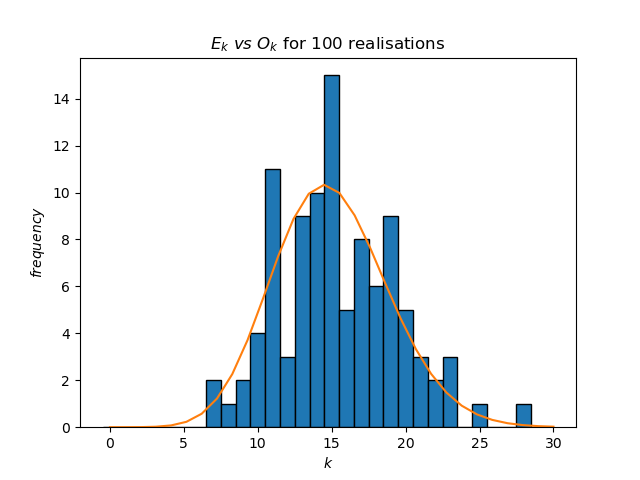
\includegraphics[width=0.333\textwidth]{inc/100.png}
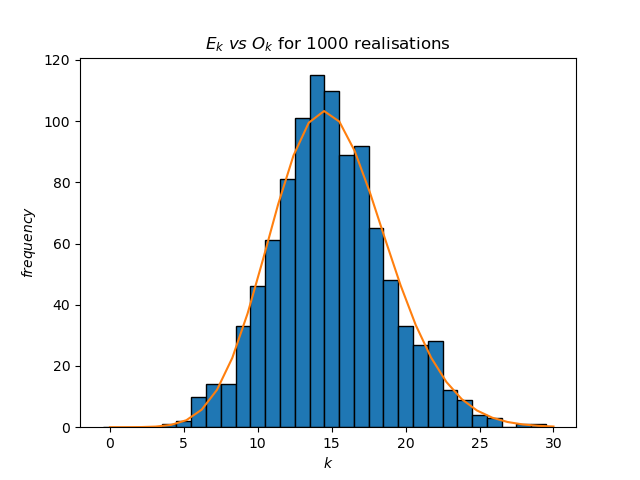
\includegraphics[width=0.333\textwidth]{inc/1000.png}
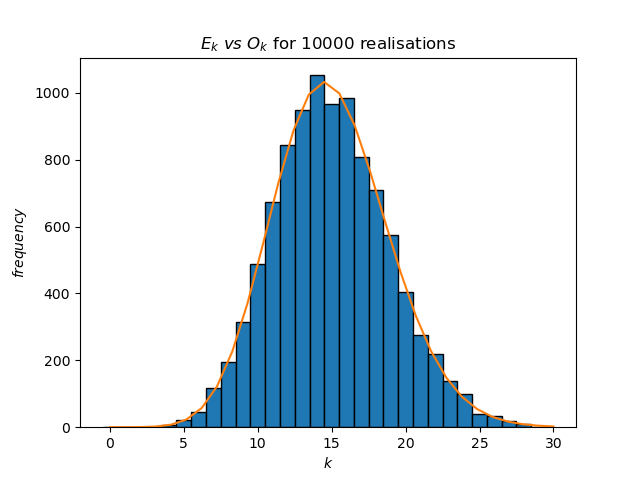
\includegraphics[width=0.333\textwidth]{inc/10000.png}
\begin{center}Figure 1.\end{center}

Figure 1 shows three runs with differing number of realisations (as histograms), overlain with theoretical distribution. Showing the general trend of greater fit for increased N. \\

\begin{center}
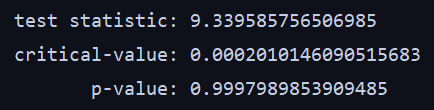
\includegraphics[width=0.333\textwidth]{inc/100_p.png}
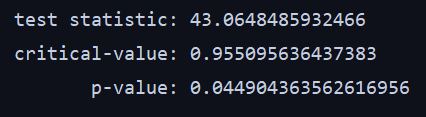
\includegraphics[width=0.3\textwidth]{inc/1000_p.png}
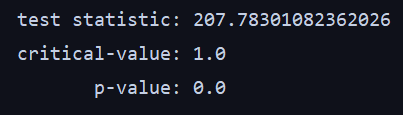
\includegraphics[width=0.3\textwidth]{inc/10000_p.png}
Figure 2.
\end{center}

Figure 2 shows the results of the $\chi^2$ test on the same differing values of N, 100, 1000, 10000.
When experimenting, I found that a N value of 2000 gave consistent results of 99\% confidence with very little outliers, at 10000 it was a constant 100\%.

When N become around 1000-1400 the critical value drops below 0.99 half the time. 

\Newpage
\section*{Appendix}
\subsection*{Part 1}
\inputpython{../py/lab4.py}{1}{60}

\end{preview}
\end{document}